

\chapter{Measure preserving systems}

\section{Measure preserving systems}
In the previous section we cheated a little bit by
considering dynamical systems without an underlying
measurable structure or notion of measure (in fact,
such a structure was implicit in the discussion of the
orbit of a ``typical'' or ``random'' initial state).
In ergodic theory we concentrate on dynamical systems
which come equipped with a measure, and furthermore,
we require the measure to be preserved under the
action of the dynamics. This idea leads to the
following definitions.

\begin{defn}
Let $(\Omega, \mathcal{F}, \mathrm{P})$ be a
probability space. A measurable map
$T:\Omega\to\Omega$ is called
$\textbf{measure preserving}$ if for any event
$E\in\mathcal{F}$ we have

\begin{equation*} \tag{13}\label{eq:measure-pres}
\mathrm{P}(T^{-1}(E)) = \mathrm{P}(E).
\end{equation*}

\noindent If $T$ is measure preserving, we say that the
probability measure $\mathrm{P}$ is \textbf{invariant under
$T$}.
\end{defn}

\noindent The condition (\ref{eq:measure-pres}) is sometimes
written in the form
$\mathrm{P}=\mathrm{P}\circ T^{-1}$. This can be
interpreted as the statement that the push-forward of
$\mathrm{P}$ under $T$ is again $\mathrm{P}$; that
is, if $X$ is an $\Omega$-valued random variable with
distribution $\mathrm{P}$, then $T(X)$ has the same
distribution.

\begin{defn}
A $\textbf{measure preserving system}$ is a
probability space equipped with a measure preserving
map, i.e., a quadruple
$(\Omega, \mathcal{F}, \mathrm{P}, T)$, where
$(\Omega,\mathcal{F},\mathrm{P})$ is a probability
space and $T:\Omega\to\Omega$ is a measure preserving
map.
\end{defn}

\noindent Measure preserving systems are the fundamental
objects studied in ergodic theory (just like vector
spaces are the fundamental objects of linear algebra,
topological spaces are the fundamental objects of
topology, etc.). It makes sense to ask to see some
examples of such systems before proceeding with their
theoretical study. Aside from some very interesting
measure preserving systems that originate in dynamical
systems (such as the billiard systems mentioned in the
previous chapter), a huge class of examples arise in a
very natural way in probability theory, and are
intimately related to the notion of a
$\textbf{stationary sequence}$, which is the subject
of the next section.

\section{Stationary sequences}
\label{sec-stationary}
Let $(X_n)_{n=1}^\infty$ be a sequence of random
variables. The sequence is called
$\textbf{stationary}$ if for any $n,m\ge 1$, we have
the equality in distribution

\begin{equation*} \tag{14}\label{eq:def-stationary}
(X_n,\ldots,X_{n+m-1}) \stackrel{\mathcal{D}}{=} (X_1,\ldots,X_m).
\end{equation*}

\noindent Note that in particular this implies that the
variables $X_1,X_2,\ldots$ are identically
distributed. Stationarity is a stronger property that
also ensures that any pair of successive variables
$(X_n,X_{n+1})$ is equal in distribution to the first
pair $(X_1,X_2)$, any triple $(X_n,X_{n+1},X_{n+2})$
is equal in distribution to the first triple
$(X_1,X_2,X_3)$, etc.; that is, any probabilistic
question about a block of adjacent variables does not
depend on the ``origin'' of the block. An i.i.d.\
sequence is a trivial example of a stationary
sequence.

A stationary sequence gives rise in a natural way to
a measure preserving system known as the
$\textbf{shift dynamics}$. To define it, first note
that although the variables may be defined on a
generic probability space
$(\Omega, \mathcal{F},\mathrm{P})$, there is no real
loss of generality in assuming that the probability
space is the $\textbf{canonical product space}$

\[
\Omega = \R^\N
\]

\noindent (sometimes denoted by $\R^\infty$) together with the
product $\sigma$-algebra
$\mathcal{B}=\mathcal{B}(R^\N)$, and the probability
measure $\mu$ defined by

\[
\mu(E) = \mathrm{P}( (X_1,X_2,\ldots) \in E ),
\]

\noindent (i.e., the distribution measure of the
infinite-dimensional vector $(X_1,X_2,\ldots)$). In
this representation, the random variables are simply
the $\textbf{coordinate functions}$

\[
X_n(\omega) = \pi_n(\omega) = \omega_n,
\]

\noindent where $\omega=(\omega_1, \omega_2, \ldots) \in \R^\N$.

On the space $(\R^\N,\mathcal{B}, \mu)$ we define the
$\textbf{shift map}$$S:\R^\N\to\R^\N$ by

\[
S(\omega_1,\omega_2, \omega_3, \ldots) = (\omega_2,\omega_3,\omega_4, \ldots).
\]

\begin{lem}
\label{lem-shift-stationary}
The shift map $S$ is a measure preserving map of the
probability space $(\R^\N,\mathcal{B},\mu)$ if and
only if the sequence $(X_n)_{n=1}^\infty$ is
stationary.
\end{lem}

\begin{xexercise}
Prove Lemma \ref{lem-shift-stationary}.
\end{xexercise}

\begin{defn}
If $(X_n)_{n=1}^\infty$ the measure preserving system
$(\R^\N,\mathcal{B},\mu,S)$ described above is called
the $\textbf{one-sided shift map}$ (or sometimes just
$\textbf{shift map}$) associated to
$(X_n)_{n=1}^\infty$.
\end{defn}

\noindent What about a two-sided shift map? One can consider a
two-sided infinite sequence
$(X_n)_{n=-\infty}^\infty$, and say that it is
stationary if the equation (\ref{eq:def-stationary}) holds
for any $m\ge1$ and $n\in\Z$. One may associate with
such a stationary sequence the
$\textbf{two-sided shift dynamics}$, which is the
measure preserving system
$(\R^\Z,\mathcal{B}(\R^\Z), \mu, S)$, where as before
$\mu$ is the distribution measure of the sequence
$(X_n)_{n\in\Z}$, and $S$ is the two-sided shift,
given by

\[
S((\omega_n)_{n\in\Z}) = (\omega_{n+1})_{n\in\Z}.
\]

\noindent One may check easily that Lemma
\ref{lem-shift-stationary} remains true when replacing the
one-sided concepts of stationary sequence and shift
dynamics with their two-sided analogues.

From the definitions it may appear that the notion of
a two-sided stationary sequence is more general than
that of a one-sided shift, since half of the elements
of a two-sided stationary sequence $(X_n)_{n\in\Z}$
can be removed to give a one-sided stationary sequence
$(X_n)_{n\ge 1}$. However, in fact this is not the
case, as the next result shows.

\begin{lem}
Given a one-sided stationary sequence
$(X_n)_{n\ge 1}$, there exists a two-sided stationary
sequence $(Y_n)_{n\in\Z}$ defined on some probability
space such that
$(Y_n)_{n\ge1} \stackrel{\mathcal{D}}{=}
(X_n)_{n\ge1}$.
\end{lem}

\begin{proof}
This is a simple example of an application of the
Kolmogorov extension theorem, a useful result from
measure theory that enables one to construct measures
on infinite product spaces with prescribed
finite-dimensional marginals (see [Dur2010], section
A.3). Here, the stationarity condition
(\ref{eq:def-stationary}) determines the joint
$m$-dimensional distribution of any block
$(Y_n,\ldots,Y_{n+m-1})$ of $m$ successive random
variables in the sequence, where $m\ge1$ and $n\in\Z$.
These distributions satisfy the consistency condition
in the Kolmogorov extension theorem, and therefore are
indeed the $m$-dimensional marginals of some infinite
sequence $(Y_n)_{n\in\Z}$ defined on a single
probability space.
\end{proof}

\noindent We saw that we can associate with any stationary
sequence a measure preserving system. Going in the
opposite direction, if we start with a measure
preserving system
$(\Omega, \mathcal{F}, \mathrm{P}, T)$, any random
variable $X:\Omega\to\R$ (what we called an
\emph{observable} in the previous chapter) can be
transformed by $T$ to a new variable

\[
X\circ T = X(T).
\]

\noindent The measure preserving property implies that
$X\circ T$ is equal in distribution to $X$. By
starting with $X$ and repeatedly iterating the
transformation $T$ we get a sequence
$(X_n)_{n=1}^\infty$ given by

\[
X_n = X\circ T^{n-1}.
\]

\begin{lem}
\label{lem-mps-stationary}
$(X_n)_n$ is a stationary sequence.
\end{lem}

\begin{xexercise}
Prove Lemma \ref{lem-mps-stationary}
\end{xexercise}

\noindent The conclusion from the above discussion is that the
study of stationary sequences is roughly equivalent to
the study of measure preserving systems with a
distinguished observable, and indeed much of ergodic
theory could be developed using just the language of
stationary sequences, although this would come at
great cost to the elegance and beauty of the theory.

\section{Examples of measure preserving systems}

\begin{enumerate}[label=\arabic*.]
\item $\textbf{i.i.d. sequences.}$ As mentioned in the
previous section, any i.i.d.\ sequence is stationary
and hence has an associated shift measure preserving
system, referred to as an $\textbf{i.i.d. shift}$. In
the case when the i.i.d.\ random variables take on
only a finite number of values with positive
probability this measure preserving system is known as
a $\textbf{Bernoulli shift}$.

\item $\textbf{A shift-equivariant function of a stationary
sequence.}$
Given a stationary sequence $(X_n)_{n=1}^\infty$ and
a measurable function $F:\R^\N\to\R^\N$ one can
manufacture a new stationary sequence
$(Y_n)_{n=1}^\infty$ via the equation

\begin{equation*} \tag{15}\label{eq:shift-equivariant}
Y_n = F(X_n,X_{n+1},X_{n+2},\ldots), \qquad (n\ge 1).
\end{equation*}

\noindent The verification that $(Y_n)_n$ is stationary is easy
and is left to the reader. In this way one can
generate starting from a known stationary sequence
(e.g., an i.i.d.\ sequence) a large class of new and
interesting sequences.

\item $\textbf{Stationary finite-state Markov chains.}$ Let
$A=\{\alpha_1,\ldots,\alpha_d\}$ be a finite set. A
\textbf{finite-state Markov chain with state space $A$} is a
sequence $(X_n)_{n=0}^\infty$ of $A$-valued random
variables such that for each $n\ge0$ and
$1\le j_1,j_2,\ldots,j_{n+1}\le d$ we have that

\begin{equation*} \tag{16}\label{eq:markov-property}
\mathrm{P}(X_{n+1} = \alpha_{j_{n+1}}\,|\,X_1=\alpha_1,\ldots,X_n=\alpha_n)
=
\mathrm{P}(X_{n+1} = \alpha_{j_{n+1}}\,|\,X_n=\alpha_n).
\end{equation*}

\noindent That is, the conditional distribution of $X_{n+1}$
given the $n$ preceding values $X_1,\ldots,X_n$ is
only dependent on the value of the last observed
variable $X_n$; this property is known as the
$\textbf{Markov property}$. In most cases the chain
is also assumed to be $\textbf{time-homogoneous}$,
meaning that the expression in (\ref{eq:markov-property})
is independent of $n$. In this case, if we denote

\[
p_{i,j} = \mathrm{P}(X_{2} = \alpha_j\,|\,X_1=\alpha_i), \qquad (1\le i,j\le d),
\]

\noindent then the matrix $P = (p_{i,j})_{i,j=1}^d$ together
with the probability distribution of the initial state
$X_0$ determine the distribution of the entire
sequence. The probability $p_{i,j}$ is referred to as
the \textbf{transition probability from state $i$ to $j$},
and the matrix $P$ is called the
$\textbf{transition matrix}$ of the chain. The
distribution of $X_0$ is usually given as a
probability vector $\pi=(\pi_1,\ldots,\pi_d)$ where
$\pi_j=\mathrm{P}(X_0=j)$. It is easy to show (we
will do so later, when we study Markov chains more in
depth) that the vector
$\pi^{(n)} = (\pi_1^{(n)},\ldots,\pi_d^{(n)})$
representing the probability distribution of $X_n$ is
obtained from $\pi$ and $P$ via

\[
\pi^{(n)} = \pi P^n,
\]

\noindent the linear-algebraic result of multiplying the row
vector $\pi$ by the matrix $P$ multiplied by itself
$n$ times.

Assume now that $\pi$ is chosen to be a probability
vector satisfying the equation $\pi=\pi P$; i.e.,
$\pi$ is a left-eigenvector of the transition matrix
$P$ with eigenvalue $1$. By the above remarks, this
means that the sequence $(X_n)_n$ is a sequence of
identically distributed random variables, and
furthermore it is easy to see that $(X_n)_n$ is in
fact a stationary sequence. A Markov chain started
with such an initial state distribution is called a
$\textbf{stationary Markov chain}$. The associated
shift measure preserving system is known as a
$\textbf{Markov shift}$.

\item $\textbf{Tossing a randomly chosen coin.}$ Let
$0\le U\le 1$ be a random variable. We can define a
stationary sequence $X_1,X_2,\ldots$ by the following
``two-step experiment'': first, pick a random coin
with bias $U$; then, toss the chosen coin infinitely
many times (the coin tosses being independent of each
other), denoting the results (encoded as 0's or 1's)
by $X_1,X_2,\ldots$. Formally, we can define the
distribution of the sequence by

\[
\mathrm{P}(X_1=a_1,\ldots,X_n=a_n) = \mathbf{E}\left[U^{\sum_j a_j} (1-U)^{n-\sum_j a_j}\right], \qquad a_1,\ldots,a_n\in\{0,1\}.
\]

\noindent Note that the $X_n$'s are identically distributed (in
fact, the sequence is stationary), but \emph{not}
independent (except in the extreme case when $U$ is
a.s.\ constant); rather, they are said to be
conditionally independent given $U$.

\item $\textbf{Pólya's urn experiment.}$ Let $I_n$ be as in
Chapter 1 the indicator random variable of the event
that in Pólya's urn experiment a white ball was drawn
in the $n$th round. We proved that the distribution
of the sequence $(I_n)_{n=1}^\infty$ is invariant
under finite permutations, so in particular it is
stationary and has an associated measure preserving
shift.

\item \textbf{Rotation of the circle} (a.k.a. \textbf{$x+\alpha$ modulo
1}). Let $(\Omega,\mathcal{F},\mathrm{P})$ be the
unit interval $[0,1]$ with Lebesgue measure. One can
consider $[0,1]$ to be topologically a circle by
identifying both endpoints $0$ and $1$ as a single
point. Fix $0\le \alpha<1$. The
$\textbf{circle rotation map}$$R_\alpha:[0,1)\to[0,1)$, which rotates the circle by
a fraction $\alpha$, is defined by

\[
R_\alpha(x) = x+\alpha \textrm{\ mod\ } 1 = \begin{cases} x+\alpha & \textrm{if }x+\alpha<1, \\ x+\alpha-1&\textrm{otherwise}. \end{cases}
\]

\begin{lem}
$R_\alpha$ preserves Lebesgue measure.
\end{lem}

\begin{proof}
If $A\subset [0,1]$ is a Borel set, then

\begin{align*}
\operatorname{Leb}(R_\alpha^{-1}(A)) &=
\operatorname{Leb}\Big( \big(A\cap[0,\alpha)+1\big) \sqcup \big(A\cap[\alpha,1)-1\big) \Big) \\
&=
\operatorname{Leb}\big(A\cap[0,\alpha)+1\big)
+  \operatorname{Leb}\big(A\cap[\alpha,1)-1\big) \\ &=
\operatorname{Leb}\big(A\cap[0,\alpha)\big)
+  \operatorname{Leb}\big(A\cap[\alpha,1)\big) \\ &=
\operatorname{Leb}\Big( \big(A\cap[0,\alpha)\big) \sqcup \big(A\cap[\alpha,1)\big) \Big)
=
\operatorname{Leb}(A).
\end{align*}

\end{proof}

\item \textbf{The $2x$ mod $1$ map.} Similarly to the previous
example, the \textbf{$2x$ mod $1$ map} or
$\textbf{doubling map}$ is also defined on the
probability space $[0,1]$ with Lebesgue measure, and
is given by

\[
D(x) = 2x\textrm{ mod }1 = \begin{cases} 2x&x<\tfrac12, \\ 2x-1&x\ge\tfrac12. \end{cases}
\]

\begin{lem}
$D$ preserves Lebesgue measure.
\end{lem}

\begin{proof}
If $A\subset [0,1]$ is a Borel set, then

\[
\operatorname{Leb}(D^{-1}(A)) =
\operatorname{Leb}\left(\tfrac12 A \sqcup \left(\tfrac12 A+\tfrac12\right) \right)
= \tfrac12 \operatorname{Leb}(A)
+ \tfrac12 \operatorname{Leb}(\tfrac12+A) =
\operatorname{Leb}(A).
\]

\end{proof}

\noindent We have seen before that the measure space $[0,1]$
with Lebesgue measure is isomorphic to the product
space of an infinite sequence of i.i.d.\ unbiased coin
tosses. It is easy to see that under this isomorphism,
the doubling map translates to the shift map $S$ of
the Bernoulli sequence. So, the doubling map is really
a disguised version of the Bernoulli shift associated
with i.i.d.\ unbiased coin tosses.

\item $\textbf{The continued fraction map.}$ A well-known
fact from number theory says that any rational number
$x\in (0,1)$ has a unique
$\textbf{continued fraction expansion}$ of the form

\[
x = \frac{1}{n_1+\frac{1}{n_2+\frac{1}{n_3+\frac{1}{\ddots+\frac{1}{n_k}}}}},
\]

\noindent where $k\ge 1$, $n_1,\ldots,n_k\in \N$ and $n_k>1$.
Such an expansion is said to be finite, or
terminating. Similarly, any irrational $x\in(0,1)$
has a unique \emph{infinite} continued fraction expansion,
which takes the form

\[
x = \frac{1}{n_1+\frac{1}{n_2+\frac{1}{n_3+\frac{1}{n_4+\frac{1}{\ldots}}}}},
\]

\noindent where $n_1,n_2,n_3\ldots \in \N$. The numbers
$n_1,n_2,\ldots$ are called the $\textbf{quotients}$
of the expansion, and are analogous to the digits in
the decimal (or base-$b$) expansion of a real number.
They are computed using a process that is a natural
generalization of the Euclidean algorithm to real
numbers, namely:

\begin{align*}
n_1 &= \textrm{the number of times a stick of length $x$ ``fits'' inside a stick of length $1$}, \\
n_2 &= \textrm{the number of times a stick of length $x_2=(1-n_1x)$ fits inside a stick}\\ &\ \ \ \ \textrm{of length $x$},
\\
n_3 &= \textrm{the number of times a stick of length $x_3=(x-n_2x_1)$ fits inside a stick} \\
&\ \ \ \ \textrm{of length $x_2$}, \\
& \ \,\vdots
\end{align*}

\noindent Gauss studied in 1812 the statistical distribution of
the quotients for a number $x$ chosen uniformly at
random in $(0,1)$. In this case, since $x$ is
irrational with probability $1$ we need not worry
about terminating expansions, and can consider the
quotients $n_1, n_2, \ldots$ to be random variables
defined on the measure space $(0,1)$ equipped with
Lebesgue measure. Gauss reformulated the problem in
terms of a measure preserving system (before this
concept even existed!) now called the
$\textbf{continued fraction map}$ or
$\textbf{Gauss map}$. To see how this reformulation
works, note first that, in the computation above, the
first quotient $n_1$ can be represented in the form

\[
n_1 = \left\lfloor \frac{1}{x} \right\rfloor
\]

\noindent (where $\lfloor z \rfloor$ denotes as usual the
integer part of a real number $z$). Next, observe
that, to continue with the computation of the next
quotients $n_2,n_3,\ldots$, instead of replacing the
two yardsticks of lengths $1$ and $x$ (which are used
in the computation of the first quotient $n_1$) by a
pair of yardsticks of lengths $x$ and $x_2=1-n_1 x$,
one can instead rescale the yardstick of length $x$
to be of length 1, so that the yardstick of length
$x_2$ becomes of length

\[
x'=\frac{1-n_1 x}{x} = \frac{1}{x}-n_1 = \left\{ \frac{1}{x} \right\}
\]

\noindent (where $\{z\}=z-\lfloor z\rfloor$ is the
$\textbf{fractional part}$ of $z$). The quotient $n_2$
can be computed from this rescaled value $x'$ in the
same way that $n_1$ is computed from $x$. By
continuing in this way one can obtain all the
quotients by successive rescaling operations.
Formally, define the Gauss map $G:(0,1)\to[0,1)$ and
a function $N:(0,1)\to\N$ by

\[
G(x) = \left\{ \frac{1}{x}\right\}, \qquad
N(x) = \left\lfloor \frac{1}{x}\right\rfloor.
\]

\noindent Then the above comments show that the quotients
$n_1,n_2,\ldots$ are obtained by

\begin{align*}
n_1 &= N(x), \\
n_2 &= N(G(x)), \\
n_3 &= N(G^2(x)), \ \ldots \\
n_k &= N(G^{k-1}(x)), \ \ldots
\end{align*}

\noindent (Note that the range of $G$ is $[0,1)$ instead of the
open interval $(0,1)$ since $G(x)=0$ exactly when $x$
is a rational number of the form $x=1/m$; this is
related to the fact that if we start with any rational
number $x$, after a finite number of iterations of $G$
we will reach $0$ and will not be able to extract any
more quotients.)

If you guessed that the Gauss map $G$ preserves
Lebesgue measure, you guessed wrong. The real
situation is more interesting:

\begin{lem}
\label{lem-gauss-measure}
The map $G$ preserves the $\textbf{Gauss measure}$$\gamma$ on $(0,1)$, given by

\[
\gamma(A) = \frac{1}{\log 2} \int_A \frac{dx}{1+x}.
\]

\end{lem}

\begin{xexercise}
Prove Lemma \ref{lem-gauss-measure}.
\end{xexercise}

\noindent An important observation is that Gauss measure and
Lebesgue measure are mutually absolutely continuous
with respect to each other. This means that any event
which has probability $1$ with respect to one is also
a probability 1 event with respect to the other. Thus
any almost-sure statistical results about the measure
preserving system $((0,1),\mathcal{B},\gamma,G)$
(which will be obtained from the Birkhoff ergodic
theorem once we develop the theory a bit more) will
translate immediately to statements about the behavior
of the continued fraction expansion of a \emph{uniformly
random} real number.

The continued fraction map described above is
intimately related to the Euclidean algorithm for
computing the greatest common divisor (GCD) of two
integers, since iterating the map starting from a
rational fraction $p/q$ reproduces precisely the
sequence of quotients (and remainders, if one takes
care to record them) in the execution of the Euclidean
algorithm, and the last non-zero iteration $T^k(p/q)$
is of the form $1/d$, where $d$ is precisely the GCD
of $p$ and $q$. Given the usefulness of the Euclidean
algorithm and its historical status as one of the
earliest algorithms ever described, is not surprising
that already in the early days of the theory of
algorithms (a.k.a.\ the 1960's) researchers were
interested in giving a quantitative analysis of the
running time of this venerable procedure. Such
analyses lead directly to ergodic theoretic questions
about the continued fraction map; the renewed interest
in this classical problem has stimulated new and
extremely interesting studies into the mathematics of
the Gauss map. A highly readable account of these
fascinating developments (the latest of which being
less than 15 years old and still inspiring new
research even in recent years) is told in
Sections~4.5.2--4.5.3 of Vol.~II of Donald E.\ Knuth's
celebrated book series \emph{The Art of Computer
Programming}.

\item $\textbf{The binary GCD algorithm.}$ Continuing the
discussion above, a fact that is little-known outside
computer science circles is that in modern times a new
algorithm for computing GCD's was proposed that gives
the Euclidean algorithm a serious run for its money,
and is actually faster in some implementations. This
algorithm was proposed by Josef Stein in 1967 and is
known as $\textbf{the binary GCD algorithm}$ or
$\textbf{Stein's algorithm}$. It replaces the integer
division operations of the Euclidean algorithm, which
are costly in some computer architectures, with a
clever use of subtractions (which are generally cheap)
and divisions by 2, which can be implemented in
machine language as (also cheap) bit shift operations.

[Here is a summary of the algorithm: start with two
integers $u<v$. First, extract the common power-of-$2$
factor to get to a situation where at least one of
$u,v$ is odd. Then, successively replace $(u,v)$ with
the new pair $(v-u)/2^k,u$ (sorted so that the
smaller one gets called ``$u$'' and the bigger one
``$v$''), where $2^k$ is the maximal power of 2
dividing $v-u$. Eventually one of the numbers becomes
$0$ and the remaining one represents the odd
component of the GCD of the original numbers.]

The computer scientist Richard Brent noticed in 1976
that this algorithm can also be reformulated in terms
of a dynamical system. Similarly to the case of the
Euclidean algorithm, the theoretical analysis of the
running time of the binary GCD algorithm leads to
highly nontrivial questions (most of them still open)
about the behavior of this dynamical system. In
particular, this system has an invariant measure that
is mutually absolutely continuous with respect to
Lebesgue measure, and is analogous to the Gauss
measure, but no good formula for it is known. See
Section~4.5.3 in Knuth's book mentioned above for more
details.

\item \textbf{The $3x+1$ map.} The \textbf{3x+1 problem} or
$\textbf{Collatz problem}$ is a famous open problem
(studied since the 1950's, and originating in work of
L.~Collatz around 1932) about a discrete dynamical
system on the positive integers. It pertains to
iterations of the map $T:\N\to\N$ defined by

\[
T(n) = \begin{cases} 3n+1 & \textrm{if $n$ is odd}, \\ \frac{\displaystyle n}{\displaystyle 2} & \textrm{if $n$ is even}.
\end{cases}
\]

\noindent The conjecture is that for any initial number $n_0$,
iterating the map will eventually lead to the cycle
$1,4,2,1,4,2,1,\ldots$ The mathematician Paul Erdös
was quoted as saying ``Mathematics is not yet ready
for such problems'' and offered a \(\$500\) prize for
its solution.

One of the many (ultimately unsuccessful) attempts to
study the problem was based on the beautiful
observation that this dynamical system can be turned
into a measure preserving system, by extending its
domain of definition to the ring $\textbf{Z}_2$ of
\textbf{$2$-adic integers}. This is an extension of the
usual ring $\Z$ of integers in which every element
has a binary expansion that extends \emph{infinitely far to
the left} (instead of to the right as a real number
would). That is, a dyadic integer is a formal
expression of the form

\[
a_0 + 2\cdot a_1 + 4\cdot a_2 + 8\cdot a_3 + \ldots + 2^n a_n + \ldots = \sum_{n=0}^\infty a_n 2^n
\]

\noindent where $a_0,a_1,a_2,\ldots\in \{0,1\}$. It can be
shown that one can do algebra, and even an exotic form
of calculus, on these numbers (and more generally over
similar sets of numbers in which the binary expansion
is replaced by a base-$p$ expansion where $p$ is an
arbitrary prime number --- these are the so-called
\textbf{$p$-adic integers}). Since the notion of the parity
of a number extends to $2$-adic integers, the $3x+1$
map $T$ extends in an obvious way to a map
$\tilde{T}:\mathbf{Z}_2\to\mathbf{Z}_2$. It can be
shown that $\tilde{T}$ preserves the natural volume
measure of $\textbf{Z}_2$. For more information, see
Wikipedia or the article \emph{The $3x+1$ problem and its
generalizations}, by J.~C.~Lagarias (\emph{American Math.
Monthly} 92 (1985), 3--23).

\item $\textbf{Billiards.}$ In Chapter 5 we discussed
billiard dynamical systems, and mentioned a formula on
the limiting statistics of such a system, in the case
when it is ergodic. This is related to the fact that
the billiard dynamics also has an invariant measure,
given (in a suitable parametrization of the phase
space) by

\[
\mu(A) = \iiint_A \frac{\sin \theta}{\sin\theta_1} \,d\theta\,d\phi\,d\ell.
\]

\item $\textbf{Hamiltonian flow.}$$\textbf{Hamiltonian mechanics}$ is a formalism for
modeling a mechanical system of particles and rigid
bodies interacting via physical forces, with no
external influences. The phase space is some set
$\Omega$ representing the possible states of the
system (formally, it is a
$\textbf{symplectic manifold}$, and has a smooth
structure --- i.e.,  one can solve differential
equations on it and do other calculus-type
operations). The $\textbf{Hamiltonian flow}$ is a
semigroup of maps $(H_s)_{s\ge 0}$ representing the
time-evolution of the system, i.e., $H_s(\omega)$
takes an initial state $\omega\in\Omega$ of the
system and returns a new state representing the state
of the system $s$ time units in the future. A result
known as Liouville's theorem says that the natural
volume measure of the manifold is preserved under the
Hamiltonian system. Thus, the Hamiltonian flow is a
$\textbf{measure preserving flow}$ (the
continuous-time analogue of a measure preserving
system, which we will not discuss in detail). Such
flows provided some of the original motivation for
questions of ergodic theory, since, e.g., statistical
physicists in the 19th century wanted to understand
the statistical behavior of ideal gases (note that
billiard can be thought of a toy model for a gas in an
enclosed region).

\item $\textbf{Geodesic flow.}$ On a compact Riemann
surface (or more generally a Riemannian manifold), the
geodesic flow $(\varphi_s)_{s\ge0}$ is a family of
maps, where each $\varphi_s$ takes a point on the
manifold together with a ``direction'' at $s$
(formally, an element of the tangent space at $s$),
and returns a new pair ``point+direction'' that is
obtained by proceeding $s$ units of distance along
the unique geodesic curve originating from $s$ in the
given direction. (For a more formal description, see
Wikipedia or a textbook on differential geometry). The
geodesic flow preserves the volume measure and is thus
a measure preserving flow.

\item $\textbf{The logistic map.}$ The logistic map was
originally studied as a simple model for the dynamics
of population growth of animal and plant species. It
is given by the formula

\[
L_r(x) = rx(1-x) \qquad (0<x<1),
\]

\noindent where $r>0$ is a parameter of the system. Here, $x$
represents the size of the population, and $L_r(x)$
represents the size of the population one generation
later, so successive iterations $L_r^{n}(x)$
correspond to the evolution of the population sizes
over time starting from some initial size $x$. The
assumptions underlying the model are that when $x$ is
small one should observe roughly exponential growth
when iterating the map, but as the size of the
population increases, the environmental resources
required to support growth are depleted, leading to
starvation and a sharp decrease in the population
size.

The logistic map is a famous example of the emergence
of $\textbf{chaos}$: for values of $r$ between $0$
and $3$, the system stabilizes around a unique value
($0$ if $r\le 1$, or $(r-1)/r$ if $1\le r\le 3$).
When $r$ becomes slightly bigger than 3 a
$\textbf{bifurcation}$ occurs, leading to an
oscillation between 2 values; as $r$ increases
further, additional bifurcations occur (oscillation
betweeen 4 values, 8 values etc.) until chaotic
behavior emerges at $r\approx 3.57$  and continues
(with occasional intervals of stability) until $r=4$,
after which point the range of the map leaves $[0,1]$
so the model stops making sense as a dynamical system.
See Figure 5 for an illustration of this remarkable
phenomenon.

\begin{center}
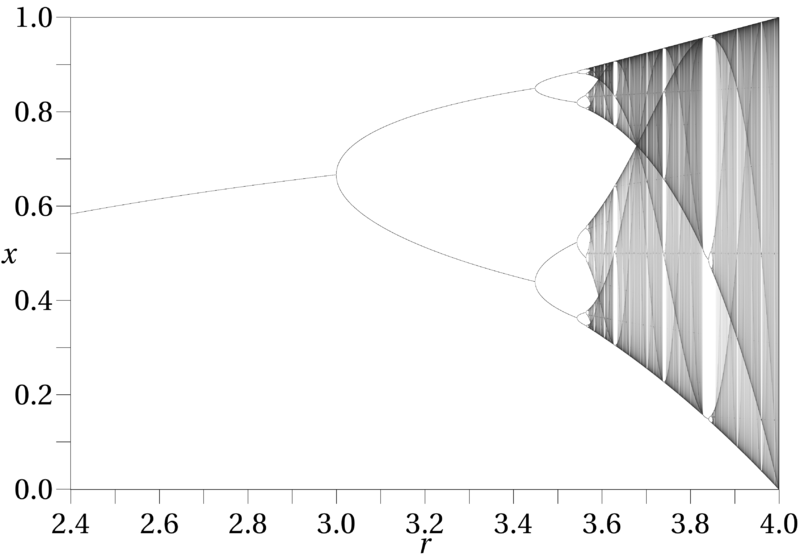
\includegraphics[width=0.70\linewidth]{figures/logisticmap.png}\\[0.6em]
{\small Figure 5: Chaos in the logistic map (source:
Wikipedia)}
\end{center}

\begin{lem}
\label{lem-logistic-invariant}
When $r=4$, the map $L_4$ has an invariant measure
$\lambda$ on $(0,1)$ given by

\[
\lambda(dx) = \frac{1}{\pi \sqrt{x(1-x)}}\,dx
\]

\noindent (also known as the
$\operatorname{Beta}(\tfrac12,\tfrac12)$
distribution).
\end{lem}

\begin{xexercise}
Prove Lemma \ref{lem-logistic-invariant}
\end{xexercise}
\end{enumerate}

\section{Ergodicity}
Let $(\Omega, \mathcal{F}, \mathrm{P}, T)$ be a
measure preserving system. An event $A\in\mathcal{F}$
is called \textbf{$T$-invariant} (or \textbf{invariant under $T$},
or just $\textbf{invariant}$ if the context is clear)
if

\[
T^{-1}(A) = A \ \ \textrm{a.s.},
\]

\noindent with the convention that two events $A,B$ are
considered equal almost surely if their symmetric
difference has probability $0$. That is, $A$ is
invariant if

\[
\mathrm{P}(A\triangle T^{-1}(A)) = 0,
\]

\noindent (where
$A\triangle B = (A\setminus B)\cup (B\setminus A)$
denotes the symmetric difference of two sets). We
denote by $\mathcal{I}$ the collection of a.s.\
invariant events.

\begin{lem}
\label{lem-invariant-sigmaalg}
$\mathcal{I}$ is a $\sigma$-algebra.
\end{lem}

\begin{xexercise}
Prove Lemma \ref{lem-invariant-sigmaalg}.
\end{xexercise}

\begin{defn}
The measure preserving system
$(\Omega, \mathcal{F}, \mathrm{P}, T)$ is called
$\textbf{ergodic}$ if for any invariant event $A$,
$\mathrm{P}(A)=0$ or $\mathrm{P}(A)=1$.
\end{defn}

\noindent A sub-$\sigma$-algebra of $\mathcal{F}$ all of whose
events have probability 0 or 1 is called
$\textbf{trivial}$. (We already saw an example: the
$\sigma$-algebra of tail events of an i.i.d.\
sequence of random variables is trivial, according to
the Kolmogorov 0-1 law.) So, another way of saying
that a measure preserving system is ergodic is that
its $\sigma$-algebra $\mathcal{I}$ of invariant
events is trivial.

There is an equivalent way to characterize ergodicity
in terms of invariant random variables rather than
events, given in the following exercise.

\begin{xexercise}
If $(\Omega, \mathcal{F}, \mathrm{P}, T)$ is a
measure preserving system, a random variable
$X:\Omega\to\R$ is called $\textbf{invariant}$ if
$X\circ T \equiv X$ almost surely. Prove that a
random variable is invariant if and only if it is
measurable with respect to $\mathcal{I}$, and that a
system is ergodic if and only the only invariant
random variables are almost surely constant.
\end{xexercise}

\begin{xexercise}
Show that a measure preserving system
$(\Omega, \mathcal{F}, \mathrm{P}, T)$ is ergodic if
and only if the probability measure $\mathrm{P}$\emph{cannot} be represented in the form

\[
\mathrm{P} = \alpha Q_1 + (1-\alpha)Q_2,
\]

\noindent where $0<\alpha<1$ and $Q_1, Q_2$ are two distinct
$T$-invariant probability measures on the measurable
space $(\Omega, \mathcal{F})$. (In words, this means
that an ergodic system cannot be decomposed into a
nontrivial convex combination of two simpler systems.)
\end{xexercise}

\noindent To get a feel for this new concept, let us examine
which of the measure preserving systems discussed in
the previous section are ergodic.

\begin{enumerate}[label=\arabic*.]
\item $\textbf{i.i.d. sequence.}$ Let $A$ be an invariant
event in the i.i.d.\ shift. $A$ is in the product
$\sigma$-algebra, in other words, it is measurable
with respect to $\sigma(X_1,X_2,\ldots)$, where
$X_1,X_2,\ldots$ denote the coordinate functions of
the product space. Then

\[
S^{-1}(A) = \{ \omega\in \R^\N \, : \, (\omega_2,\omega_3,\ldots) \in A \}
\]

\noindent is measurable with respect to
$\sigma(X_2,X_3,\ldots)$, and similarly, for any
$n\ge 1$,

\[
S^{-n}(A) = \{ \omega\in \R^\N \, : \, (\omega_{n+1},\omega_{n+2},\ldots) \in A \}
\]

\noindent is in $\sigma(X_{n+1},X_{n+2},\ldots)$. It follows
that

\[
A'=\bigcap_{N=1}^\infty \bigcup_{n=N}^\infty S^{-n}(A) = \{ S^{-n}(A) \textrm{ i.o.} \}
\]

\noindent is a tail event, and hence has probability $0$ or $1$
by the Kolmogorov 0-1 law. But we assumed that $A$
was invariant, which implies that $A=S^{-n}(A)$
almost surely for all $n\ge 1$, and therefore also
$A=A'$ almost surely. It follows that $A$ is also a
0-1 event\footnote{The above argument shows that
$\mathcal{I}\subseteq\mathcal{T}$ (the
$\sigma$-algebra of invariant subsets is contained in
the tail $\sigma$-algebra), as long as we identify
sets which are a.s.\ equal.}. We have proved:

\begin{lem}
\label{lem-iid-ergodic}
Any i.i.d.\ shift map is ergodic.
\end{lem}

\item $\textbf{A shift-equivariant function of an ergodic
stationary sequence.}$\footnote{In more abstract treatments of ergodic theory, this
example would be called a $\textbf{factor map}$ or
$\textbf{homomorphism}$. An important family of
problems in ergodic theory is concerned with
identifying when one measure preserving system can be
obtained as a homomorphism of another (usually
simpler) measure preserving system, and especially
when one can find an \emph{invertible} homomorphism, also
known as an $\textbf{isomorphism}$, between the two
systems.}
Let $(X_n)_n$ be a stationary sequence whose
associated shift system is ergodic (such a sequence is
called simply a
$\textbf{stationary ergodic sequence}$), and let $Y_n$
be defined as in (\ref{eq:shift-equivariant}).

\begin{lem}
The stationary sequence $(Y_n)_n$ is also ergodic.
\end{lem}

\begin{proof}
Let $A$ be an invariant event for the $(Y_n)$
sequence. We can think of $A$ as ``living'' in the
original product space $\R^\N$ associated with the
shift map for the sequence $(X_n)_n$. (Formally, the
sequence $(Y_n)_n$ is an infinite-dimensional random
vector, i.e., it maps the $\R^\N$ ``of'' the $(X_n)_n$
sequence into a ``different copy'' of $\R^\N$; by
pulling back the event $A$ with respect to this
mapping we get a ``copy'' of $A$ in the original
product space.) The fact that $A$ is invariant under
shifting the $Y_n$'s means it is also invariant under
the original shift of the $X_n$'s, hence is a 0-1
event by the assumption that the $(X_n)_n$ sequence
is ergodic.
\end{proof}

\item $\textbf{Stationary finite-state Markov chains.}$ A
Markov chain is called $\textbf{irreducible}$ if any
state can be reached in a sequence of steps from any
other state. It is not hard to prove (see [Dur2010,
Example~7.1.7, p.~281]) that a stationary finite-state
Markov chain is ergodic if and only if it is
irreducible.

\item $\textbf{Tossing a randomly chosen coin.}$ In this
experiment we have

\[
U = \lim_{n\to\infty} \frac{1}{n}\sum_{k=1}^n X_k
\]

\noindent by the strong law of large numbers (conditioned on
the value of $U$). So, the random coin bias $U$ is an
invariant random variable, and thus the sequence
$(X_n)_n$ is ergodic if and only if $U$ is a.s.\
constant (equivalently, if and only if the sequence is
i.i.d.).

We should note that this process is in some sense an
archetypical example of a non-ergodic process, in the
sense that non-ergodicity is precisely the behavior in
which the experiment chooses ``at the dawn of time''
some random data or information (represented by the
$\sigma$-algebra of invariant events), and then
performs a stationary ergodic sequence of experiments
that depends on this initial data. In other words, a
general stationary sequence can always be represented
as a mixture, or a kind of weighted average, of
stationary ergodic sequences, where the weights in the
mixture correspond to the probability distribution of
the initial data. (The precise formulation of this
statement leads to the concept of the
$\textbf{ergodic decomposition}$ of a measure
preserving system, which we will not discuss in detail
since it requires some slightly advanced notions from
functional analysis.)

\begin{xexercise}
Show that the $\sigma$-algebra $\mathcal{I}$ of
invariant subsets for this process coincides with the
$\sigma$-algebra $\sigma(U)$ generated by the random
coin bias $U$. That means that, not only is $U$ an
invariant random variable, but any other invariant
random variable can be computed once the value of $U$
is known.
\end{xexercise}

\item $\textbf{Pólya's urn.}$ The limiting fraction $Y$ of
white balls in the urn (see (\ref{eq:polya-as-conv})) is
an invariant random variable. By
(\ref{eq:polya-beta-dist}), it is non-constant, which
shows that the shift associated  with the stationary
sequence of indicators $(I_n)_n$ in Pólya's urn
experiment is not ergodic.

It is an amusing and rather counter-intuitive fact
that the Pólya urn experiment is actually a special
case of the ``tossing a randomly chosen coin'' family
of examples discussed above. In fact, the ``random
coin bias'' $U$ is equal to the limiting fraction $Y$
of white balls in the urn. To see this, note that by a
short computation (\ref{eq:polyaurn-formula}) can be
massaged into the form

\[
\mathrm{P}(I_1=x_1, \ldots, I_n=x_n) = \frac{B(a+k, b+n-k)}{B(a,b)},
\]

\noindent where $B(u,v)=\int_0^1 x^{u-1}(1-x)^{v-1}\,dx$
denotes the Euler beta function, and
$k=\sum_{j=1}^n x_j$ (check!). We can further
recognize the quantity on the right hand side as an
expectation, namely

\[
\frac{B(a+k, b+n-k)}{B(a,b)}= \frac{1}{B(a,b)}\int_0^1 x^{a-1}(1-x)^{b-1} x^k(1-x)^{n-k}\,dx = \mathbf{E}(U^k(1-U)^{n-k}),
\]

\noindent where $U\sim \operatorname{Beta}(a,b)$. Thus, we have
the amazing fact that, in effect, Pólya's urn behaves
as if at the beginning of time, it \emph{chooses} the
random limiting fraction $Y$ of white balls (without
telling the experimenter!), and subsequently tosses an
i.i.d.\ sequence of coin tosses with bias $Y$ to
choose the successive colors of the balls that get
added to the urn. Furthermore, by the exercise above,
the $\sigma$-algebra of invariant subsets is the one
generated by $Y$, so intuitively one can say that
this random variable measures the precise extent of
non-ergodicity in the process, i.e., the decomposition
of the process into its ergodic components.

\item $\textbf{Rotation of the circle.}$ The following
result has a natural number theoretic interpretation,
which we'll discuss later after proving the Birkhoff
pointwise ergodic theorem.

\begin{thm}
The circle rotation map $R_\alpha$ is ergodic if and
only if $\alpha$ is irrational.
\end{thm}

\begin{proof}
If $\alpha=p/q$ is rational, the set

\[
E = \left[0, \tfrac{1}{2q}\right]
\cup \left[\tfrac{1}{q}, \tfrac{3}{2q}\right]
\cup \left[\tfrac{2}{q}, \tfrac{5}{2q}\right]
\cup \left[\tfrac{3}{q}, \tfrac{7}{2q}\right]
\cup \ldots
\cup \left[\tfrac{q-1}{q}, \tfrac{2q-1}{2q}\right]
\]

\noindent is an example of a nontrivial invariant set.
Conversely, assume that $\alpha$ is irrational. Let
$A \subset [0,1]$ be an invariant event. The
indicator variable $\mathbf{1}_A$ is a bounded
measurable function, hence an element of $L_2[0,1]$,
and can therefore be expanded in the Fourier basis

\[
\mathbf{1}_A(x) = \sum_{n=-\infty}^\infty c_n e^{2\pi inx}.
\]

\noindent (The equation represents an equality in $L_2$, i.e.,
it is true for almost every $x\in [0,1]$.) The
coefficients $c_n$ in the expansion are given by
$c_n = \frac{1}{2\pi} \int_0^1 \mathbf{1}_A(x)
e^{-2\pi i n x}\,dx$.
Then we have

\begin{align*}
\mathbf{1}_{R_\alpha^{-1}(A)}(x) &= (\mathbf{1}_A\circ R_\alpha)(x) = \mathbf{1}_A(R_\alpha(x))
= \sum_{n=-\infty}^\infty c_n e^{2\pi i n R_\alpha(x)}
= \sum_{n=-\infty}^\infty c_n e^{2\pi i n (x+\alpha\textrm{ mod }1)} \\
&
= \sum_{n=-\infty}^\infty c_n e^{2\pi i n (x+\alpha)}
= \sum_{n=-\infty}^\infty d_n  e^{2\pi i n x},
\end{align*}

\noindent where we denote $d_n = c_n e^{2\pi in\alpha}$. Since
$A$ is invariant, i.e.,
$\mathbf{1}_{R_\alpha^{-1}(A)}=\mathbf{1}_A$ a.s., we
get that $c_n=d_n$ for all $n\in\Z$. But $\alpha$ is
irrational, so $e^{2\pi in\alpha}\neq 1$ if $n\neq 0$.
It follows that $c_n=0$ for all $n\neq 0$, which
leaves only the constant Fourier coefficient, i.e.,
$\mathbf{1}_A \equiv c_0$ a.s., which proves that $A$
is a trivial event.
\end{proof}

\item \textbf{The $2x\textrm{ mod }1$ map.} As we discussed
earlier, this system is equivalent to the
$(\tfrac12,\tfrac12)$ Bernoulli shift, so by Lemma
\ref{lem-iid-ergodic} above, the doubling map is ergodic.

\item $\textbf{The continued fraction map.}$ The Gauss map
is ergodic, a fact which has important consequences
(which we will discuss in the next chapter) for
understanding the distribution of continued fraction
quotients of a typical real number. There are many
proofs of this result. See for example the book
\emph{Ergodic Theory and Information} by P.\ Billingsley,
and the paper by Bowen cited in example 13 below.

\item \textbf{The $3x+1$ map.} K.\ R.\ Matthews and A.\ M.\ Watts
studied the extension $\tilde{T}$ of the $3x+1$ map
to the $2$-adic integers in a 1983 paper, and in
particular proved that $\tilde{T}$ is ergodic (see
the survey by Lagarias mentioned in Section 6.3).

\item $\textbf{Billiards.}$ In Chapter 5 we described some
example of billiard systems which are known to be
ergodic, and some which aren't (for relatively trivial
reasons). In general it is extremely difficult to
prove that a given billiard system is ergodic, but,
similarly to the example of Markov chains described
above, there is a kind of philosophical principle
(that applies to billiard and other types of dynamical
systems) that says that unless a system is non-ergodic
for a relatively obvious or trivial reason (e.g.,
because there is some obvious quantity that is
conserved such as the energy of a mechanical system),
one would expect the system to be ergodic, even though
in practice one may have no idea how to prove it in a
given situation. As with any philosophical principle,
one should take care in deciding how to apply
it\footnote{Note: a \emph{philosophical principle} is what
mathematicians invent when they can't say anything
rigorous.}.

\item $\textbf{Hamiltonian flow.}$ The situation is similar
to that of billiard systems: most systems are assumed
to be ergodic unless there are obvious reasons why
they are not, but as far as I know this cannot be
proved in virtually any example which has any
real-world relevance.

\item $\textbf{Geodesic flow.}$ Some geodesic flows are not
ergodic (e.g., the sphere), and others are (for
example, hyperbolic space). The main property required
to have ergodicity is negative curvature, but I am not
familiar with the specific details. It is also
interesting to note that there is a beautiful theory
linking the continued fraction map and other dynamical
systems with a number-theoretic flavor to geodesic
flows on compact hyperbolic surfaces (in the case of
the continued fraction map, it can be related to the
geodesic flow on the $\textbf{modular surface}$$\mathbb{H}/PSL(2,\mathbb{Z})$, the quotient of the
hyperbolic plane by the modular group).

\item $\textbf{The logistic map.}$ This map is ergodic, a
fact that follows as a consequence of a much more
general result proved in the paper \emph{Invariant measures
for Markov maps of the interval}, by R.\ Bowen
(\emph{Commun. Math. Phys.} 69 (1979), 1--17).
\end{enumerate}

